\subsection{Validation}
\begin{frame}{Validation}
Validation of optimal solution can be observed directly for low dimensional searches
\begin{table}
    \caption[3 Bit Genome Results]{Bit String Simplified Geometry Descriptions}
    \label{tab:BitStringGeo}
    \centering
    \tiny
    \begin{tabular}{ p{1.5cm} | p{1.5cm} p{1.5cm}  p{1.5cm}}
			Genome&Mass Li-6&Count Rate& Count Rate per Mass \\
      \hline
      \hline
			010&16.7&2.9&0.175 \\ 
			\hline
			011&33.5&3.3&0.100 \\
			001&16.7&1.28&0.074 \\
			111&50.3&4.6&0.091 \\
			110&33.5&4.2&0.125 \\ 
			100&16.7&2.5&0.147 \\
			101&33.5&3.9&0.116 \\
      \hline
    \end{tabular}
\end{table}
Similarly for other low dimensional search spaces
\end{frame}

\begin{frame}[fragile]{Bootstrapped Genomes and Engineering Judgment}
\begin{itemize}
	\item Observed that all optimal solutions in low dimensions have moderator and reflector
	\item Possibility to reduce search space by setting moderator and reflector bits
	\item Possibility to initialize solutions for higher dimensions from lower ones
	\begin{itemize}
		\item Example: \verb+010+ $\to$ \verb+01000+ $\to$ \verb+0010000100000+
		\item Danger is not having enough diversity to avoid local minima
	\end{itemize}
\end{itemize}
\end{frame}

\begin{frame}[fragile]{Optimal Geometries}
\begin{table}
    %\caption[Optimal Bit String Geometries]{Genatic Algothrim Optimal Geometries}
    \centering
    \tiny
    \begin{tabular}{ p{0.75cm} | p{1cm} p{3.25cm} p{0.75cm} p{1cm} p{1cm}}
      Genome Length&Films Per Assembly&Optimal Geometry&Mass \iso[6]{Li}(g)&CPS per ng \iso[252]{Cf} & Count Rate per Mass \iso[6]{Li} (cps/g) \\
      \hline
      \hline
      3&4&\verb+010+&16.75&2.93&0.175 \\
      4&4&\verb+0100+& & & \\
      5&3&\verb+01000+&12.56&2.89&0.230 \\
      6&3&\verb+010000+&12.56&2.88&0.230 \\
      7&3&\verb+0100000+&12.56&2.84&0.226 \\ 
      10&3&\verb+0100000000+&12.56&2.68&0.214 \\
      10&3&\verb+0010000000+&12.56&2.93&0.233 \\
      10&3&\verb+0001000000+&12.56&2.95&0.235 \\
      13&2&\verb+00010010000000+&16.75&3.88&0.232 \\
      13&2&\verb+00100010000000+&16.75&3.90&0.233 \\
      13&2&\verb+00100100000000+&16.75&3.87&0.231 \\
      26&1&\verb+00000110110000000010000000+&20.94&4.33&0.206 \\
      26&1&\verb+00001010001000100000000000+&16.75&4.20&0.251 \\
    \end{tabular}
\end{table}
\end{frame}
%%%%%%%%%%%%%%%%%%%%%%%%%%%%%%%%%%%%%%%%%%%%%%%%%%%%%%%%%%%%%%%%%%%%%%%%%%
\begin{frame}{Optimal Geometries Rendered}
\begin{figure}
    \centering
    \begin{subfigure}[b]{0.45\textwidth}
        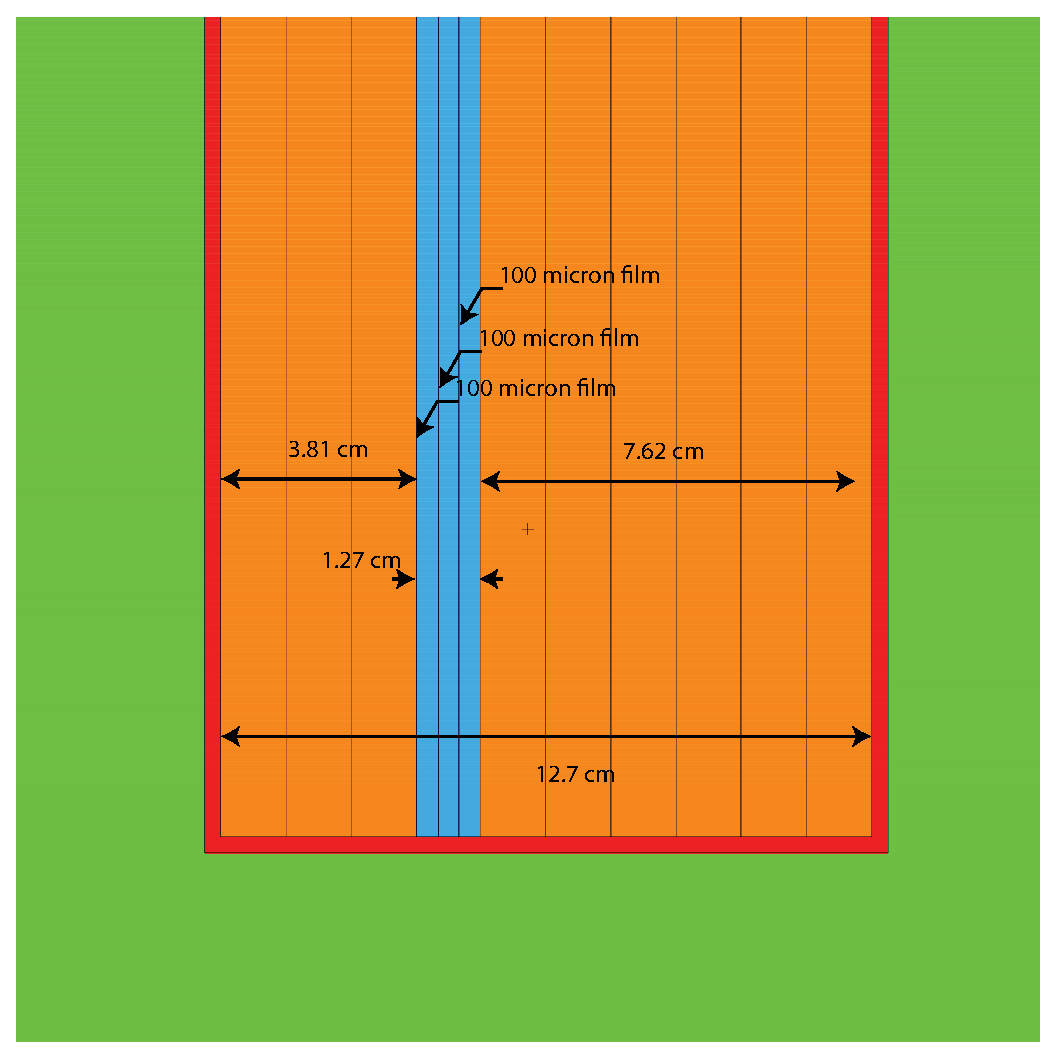
\includegraphics[width=\textwidth]{RPM8_Diagrams_MCNPXRender_10Opt}
    \end{subfigure}%
    ~
    \begin{subfigure}[b]{0.45\textwidth}
        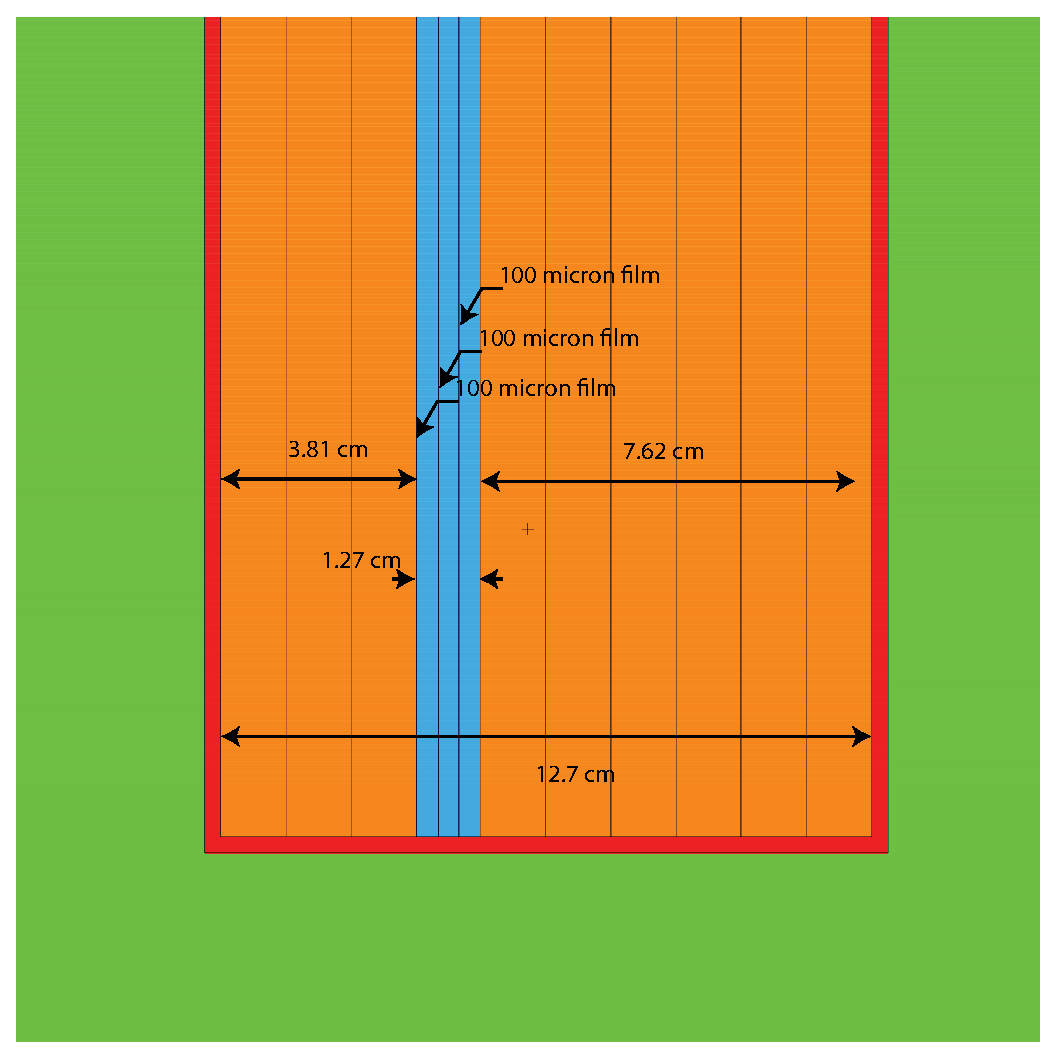
\includegraphics[width=\textwidth]{RPM8_Diagrams_MCNPXRender_26Opt}
    \end{subfigure}
    \caption{MCNPX rendering of layered geometry}
    \label{fig:MCNPXRendering}
\end{figure}
\end{frame}
%%%%%%%%%%%%%%%%%%%%%%%%%%%%%%%%%%%%%%%%%%%%%%%%%%%%%%%%%%%%%%%%%%%%%%%%%%
\subsection{Timing and Run Information}
\begin{frame}{Number of Geometries and Search Space}
Benefit of GA becomes apparent at higher search spaces!
\begin{table}
    %\caption[Optimal Bit String Geometries]{Genatic Algothrim Optimal Geometries}
    \centering
    \tiny
    \begin{tabular}{ p{0.75cm} | p{1cm} p{1cm} p{1cm} p{1cm} p{1cm}}
      Genome Length&Population Size&Number Runs&Average Generations&Fraction of Search Space Covered&Average Geometries Simulated \\
      \hline
      \hline
      3&6&20&4.6&100\%&24.5 \\
			4&8&18&3.8&100\%&30.7 \\
			5&10&18&6.0&100\%& 60.0 \\
			6&12&19&7.6&100\%&91.6 \\
			7&14&16&8.8&0.87\%&122.7 \\
			10&20&12&26.8&0.47\%& 536.7 \\
			13&26&8&19.0&0.18\% &494.0\\
			26&52&2&8.5&0.0014\% &442.0\\
    \end{tabular}
\end{table}
\end{frame}
